% !TeX root = ../main.tex
% !TEX spellcheck = en_GB

\chapter{Architecture}
\label{sec:Architecture}
This section describes the overall system architecture, the chosen platforms for development and how the different subsystems communicate with each other.
The architecture is illustrated with a Block Definition Diagram (BDD), an Internal Block Diagram (IBD) and an allocation diagram.

\begin{figure}[H]
	\centering
	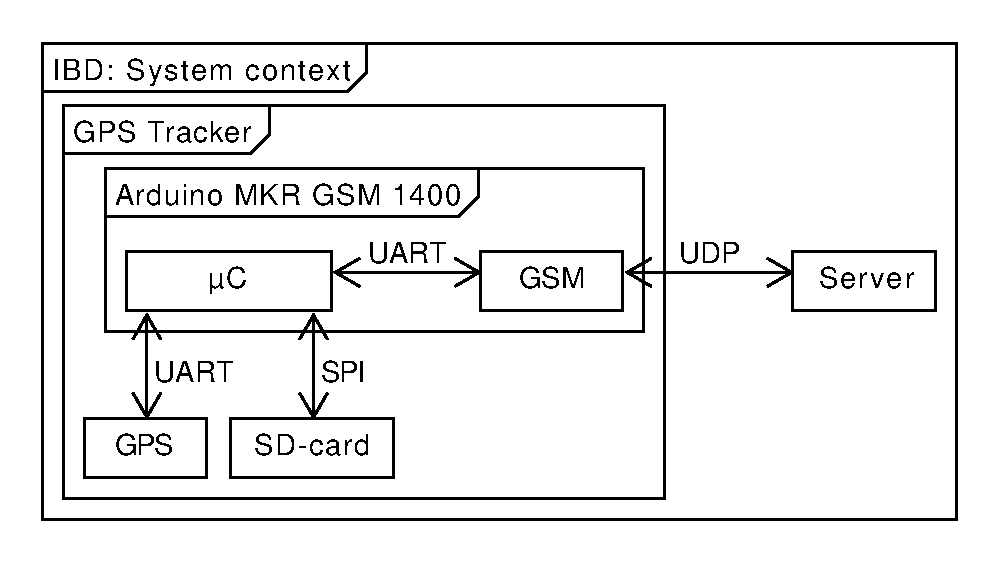
\includegraphics[width=0.7\linewidth]{gfx/Design/Overall_IBD.pdf}
	\caption{Overall BDD, including types of connection.}
	\label{fig:BDD:overall}
\end{figure}

\section{Sequence Diagrams}

\begin{figure}
	\centering
	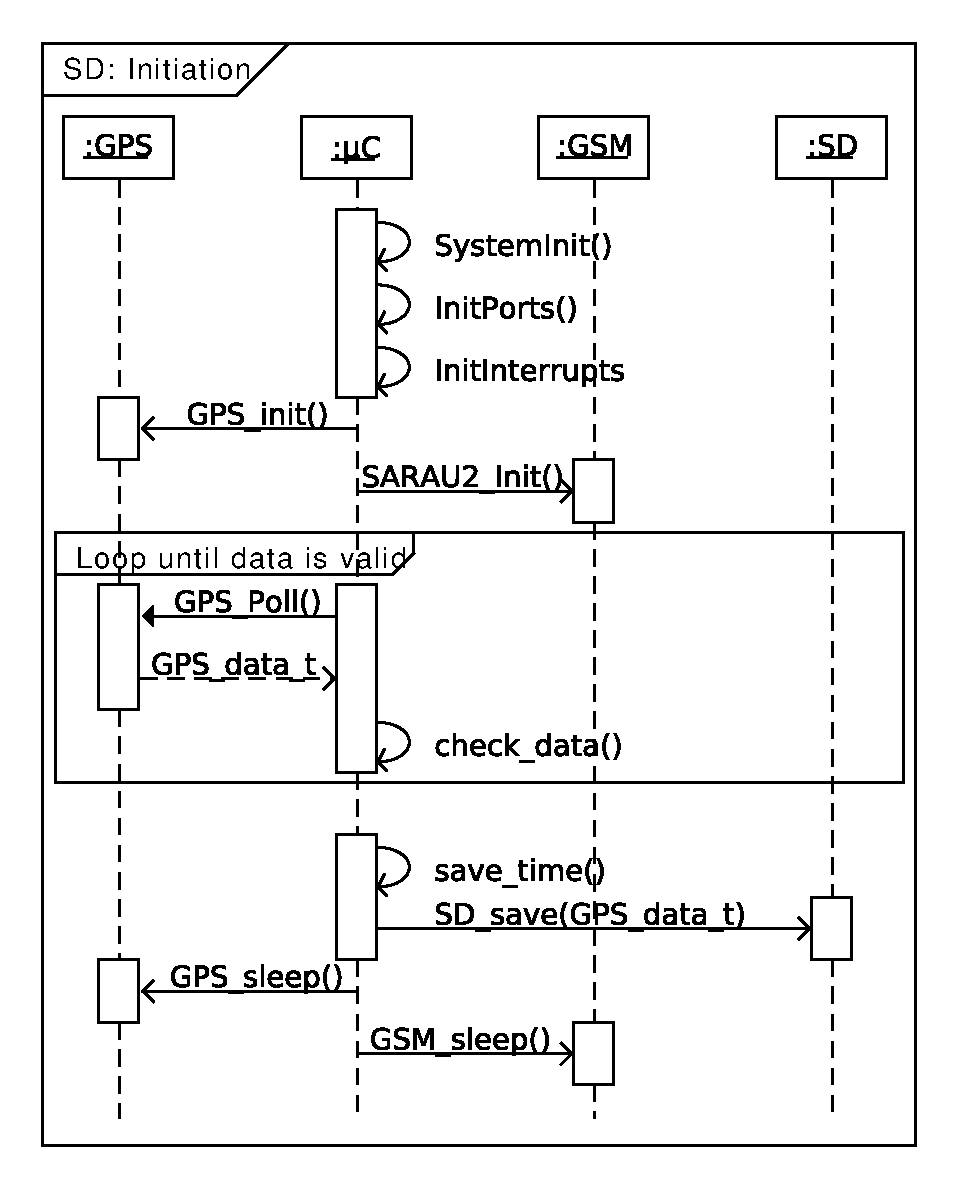
\includegraphics[width=0.7\linewidth]{gfx/Design/SD_init.pdf}
	\caption{}
	\label{fig:SD:init}
\end{figure}

\begin{figure}
	\centering
	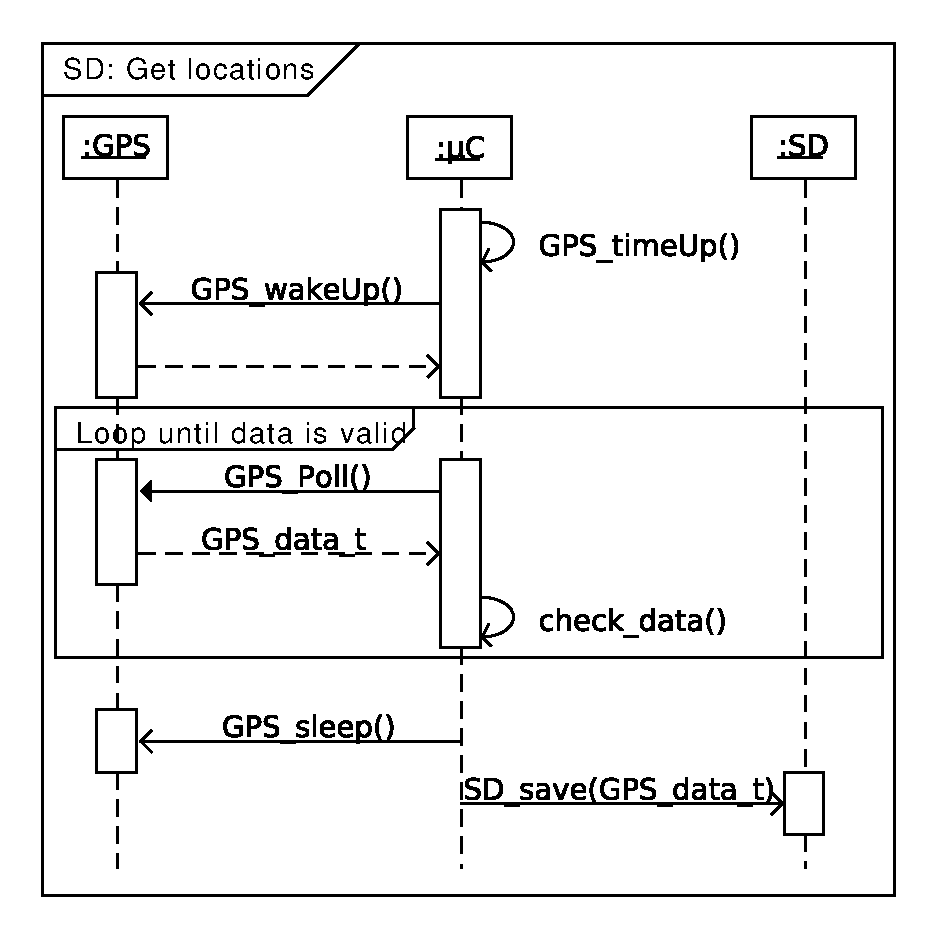
\includegraphics[width=0.7\linewidth]{gfx/Design/SD_getLocation.pdf}
	\caption{}
	\label{fig:SD:getlocation}
\end{figure}

\begin{figure}
	\centering
	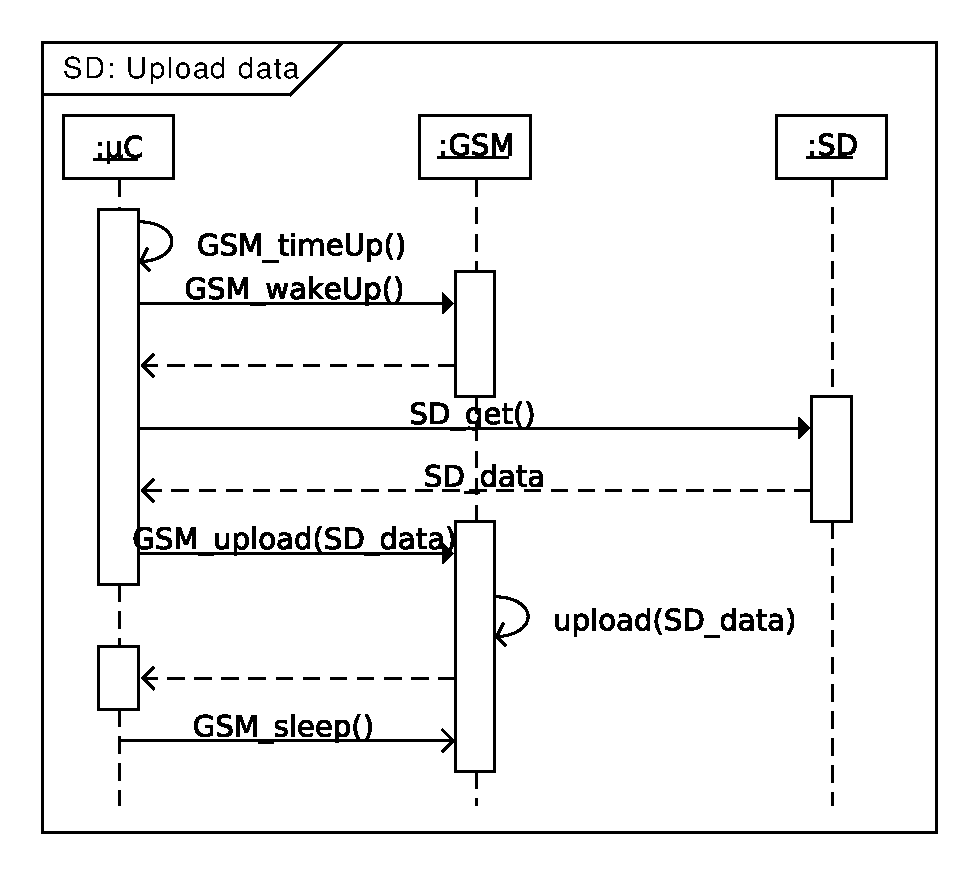
\includegraphics[width=0.7\linewidth]{gfx/Design/SD_Upload.pdf}
	\caption{}
	\label{fig:SD:upload}
\end{figure}



\FloatBarrier